\section{Introduction}
\begin{frame}
  \frametitle{Introduction}
  \begin{columns}[c]
    \begin{column}[T]{.5\textwidth}
      \begin{itemize}
        \item Pour l'Inria équipe mnemosyne
        \item Travail demandé
          \begin{itemize}
            \item Reproduire le projet Pinikio
            \item Documenter la réalisation
            \item API simple pour controler le robot
          \end{itemize}
        \item Servira pour l'étude des comportements
      \end{itemize}
    \end{column}
    \begin{column}[T]{.5\textwidth}
      \begin{figure}
        \begin{center}
          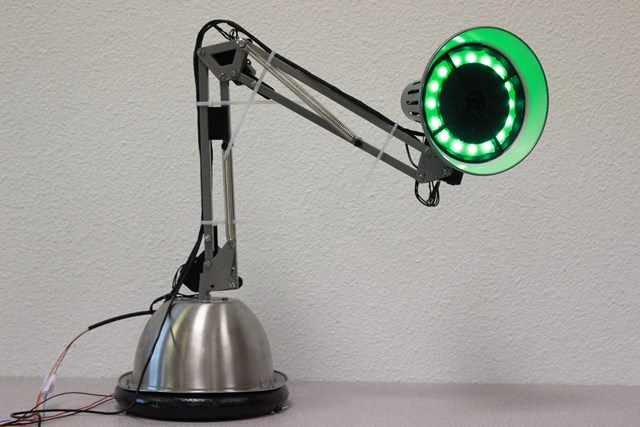
\includegraphics[width=5cm]{../img/pinokio.JPG}
        \end{center}
      \end{figure}
    \end{column}
  \end{columns}   
\end{frame}
